\chapter{The program}
When the program runs, it takes the image, and performs the image processing on it. Along the way it makes windows showing the steps visually. First step is just the input image
	\begin{figure}[H]
		\centering
		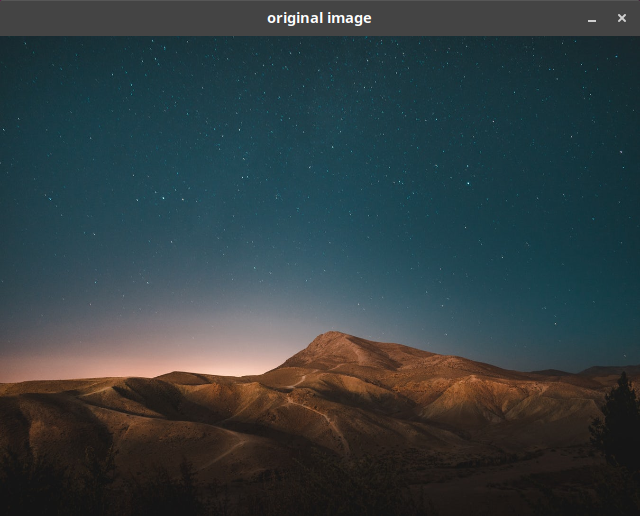
\includegraphics[width=0.6\linewidth]{figure/originalImage}
		\caption{The input image}
		\label{fig:originalImage}
	\end{figure}
	We then use the built-in opencv function to convert the image to gray scale, as this isn't strictly relevant to horizontal and vertical edge detection.
	\begin{figure}[H]
		\centering
		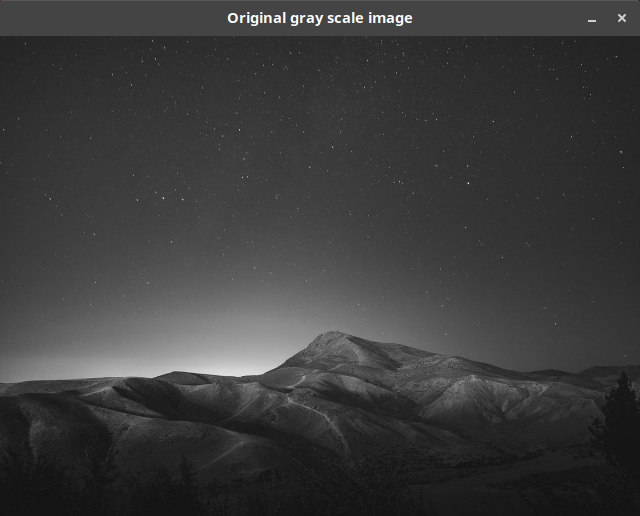
\includegraphics[width=0.6\linewidth]{figure/grayScaleImage}
		\caption{Gray scale image}
		\label{fig:grayScaleImage}
	\end{figure}
	This is then the image after the vertical edges have been detected.
	\begin{figure}[H]
		\centering
		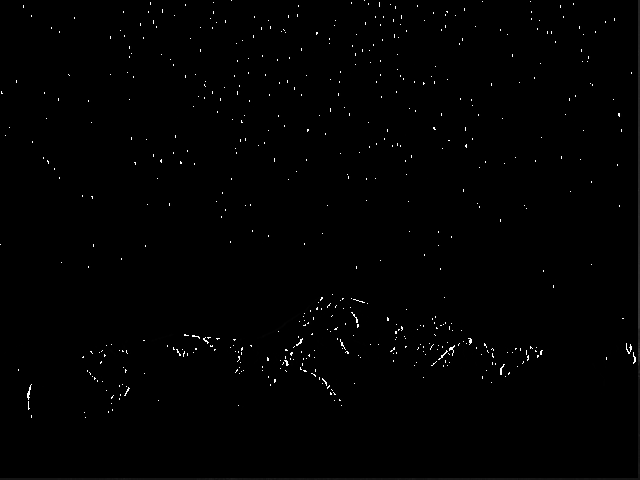
\includegraphics[width=0.6\linewidth]{figure/xEdge}
		\caption{Vertical edges detected}
		\label{fig:xEdge}
	\end{figure}
	Then there's the horizontal edges.
	\begin{figure}[H]
		\centering
		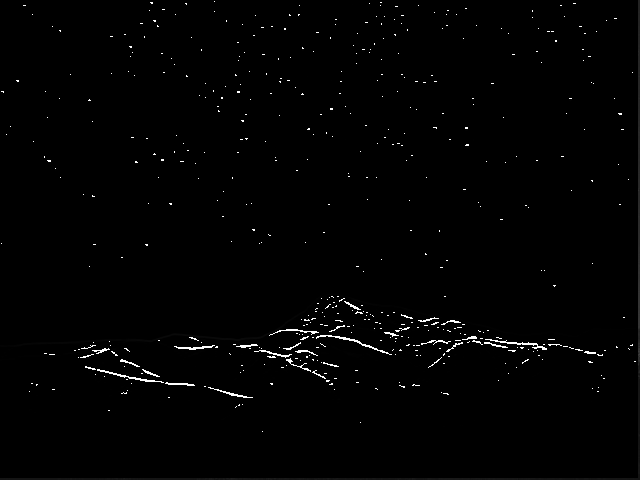
\includegraphics[width=0.6\linewidth]{figure/yEdge}
		\caption{Horizontal edges detected}
		\label{fig:yEdge}
	\end{figure}\newpage
And then there's the complete final result, with the combined images.
\begin{figure}[H]
	\centering
	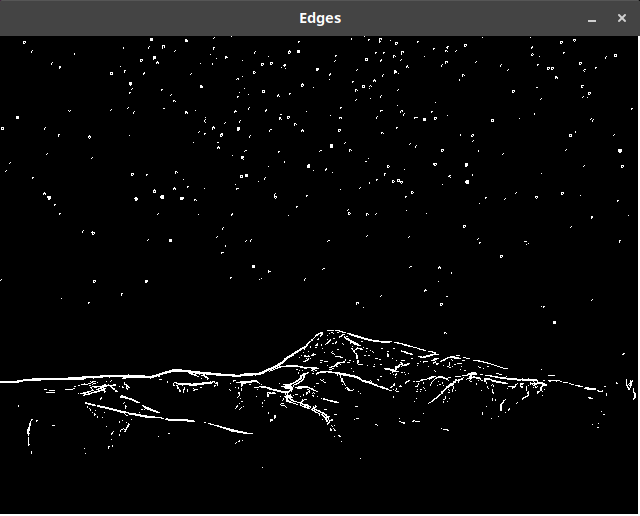
\includegraphics[width=0.6\linewidth]{figure/finalGradient}
	\caption{The resulting image, combining both from both the other images.}
	\label{fig:finalGradient}
\end{figure}

Now the two very important parts of the program is the kernels, and the amount you divide the scale by, when taking the gradients of the image.
Starting off with the scale number, I am fairly certain this is a form of simple normalization. Doubling the number from 60 to 120, makes the function much more aggressive, as seen in \autoref{fig:scale120}.
\begin{figure}[H]
	\centering
	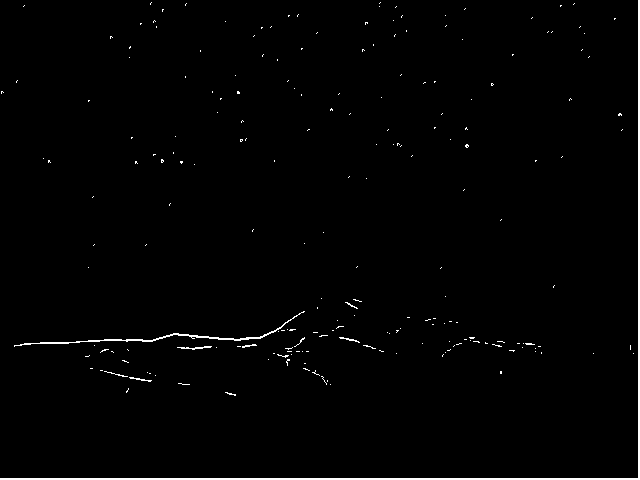
\includegraphics[width=0.6\linewidth]{figure/scale120}
	\caption{The final image, with the doubled scale divider number}
	\label{fig:scale120}
\end{figure}\newpage
Now when changing the kernel, the results change drastically. The kernel used in \autoref{fig:otherKernel} looks like this
\[
xKernel = 
\begin{bmatrix}
-3 & 0 & 3\\
-10 & 0 & 10\\
-3 & 0 & 3
\end{bmatrix},\hspace{0.7cm}
yKernel = 
\begin{bmatrix}
-3 & -10 & -3\\
0 & 0 & 0\\
3 & 10 & 3
\end{bmatrix}
\]
With the new kernel, the image is much more "detailed", and the whole mountain range line is kept intact, but much "noise" inside the mountain is also introduced.
\begin{figure}[H]
	\centering
	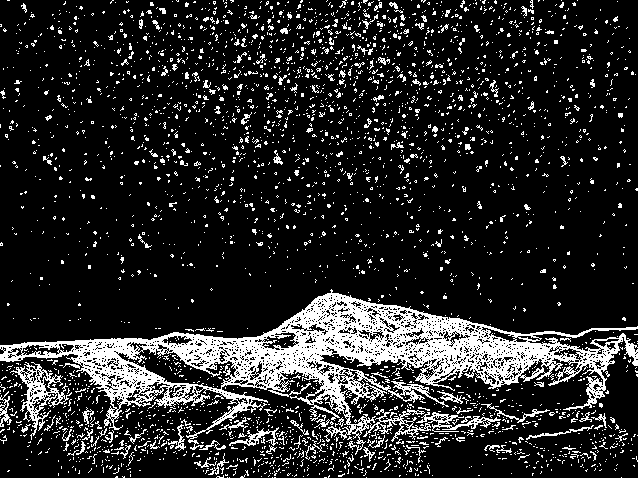
\includegraphics[width=0.7\linewidth]{figure/otherKernel}
	\caption{The final image, with another kernel}
	\label{fig:otherKernel}
\end{figure}